\documentclass[12pt,letterpaper]{report}
\usepackage[utf8]{inputenc}
\usepackage[spanish]{babel}
\usepackage{amsmath}
\usepackage{amsfonts}
\usepackage{amssymb}
\usepackage{graphicx}
\usepackage[left=2cm,right=2cm,top=2cm,bottom=2cm]{geometry}
\author{Jose Antonio Olvera Gonzalez }
\title{Descubrir los metodos geometricos, algebraico y desacoclo cinematico }
\begin{document}
\begin{center}
\textbf{Metodos Geometricos, algebraico y desacoplo}
\begin{flushleft}
Geometricos 
\begin{flushleft}
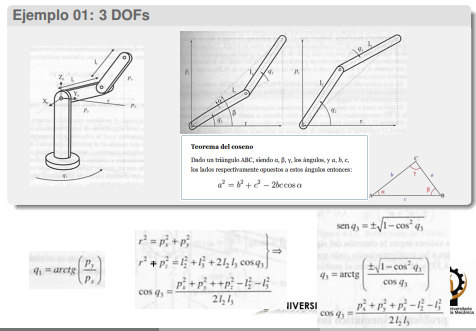
\includegraphics[scale=1]{1.PNG} 
\begin{flushleft}
Se suele utilizar para las primeras variabbles articulares uso de relaciones geometricas y trigonometricas ( resolucion de tiangulos ) .\\
Se resuelve la cinemática directa y se obtienen las matrices A. Para evitar la aparición aparición de ecuaciones ecuaciones trascendentes, trascendentes, se va
premultiplicando por las matrices inversas. Se intenta obtener de esta forma una ecuación que aísle en uno
de los lados una de las variables variables articulares articulares. La elección de los elementos ha de realizarse con sumo cuidado. Por su complejidad a menudo este método se deshecha.\\
Son útiles en robots con pocos grados de libertad (degrees of
freedom - DOFs)

\begin{flushleft}
Metodo algebraico
\begin{flushleft}
Pasos del método\\
-Identificar una solución básica factible inicial.\\
-Determinar si existe una solución básica factible mejor. Si es así, llevar a cabo el paso siguiente(3). Si no la solución actual es la óptima.\\
-Pasar a la siguiente solución básica factible, cambiando una variable no básica por una variable básica, haciendo que todas las variables sigan siendo no-negativas y regresar al paso 2.
\begin{flushleft}
Ventajas del método:\\
*Es más claro entender la razón.\\
*Se pueden resolver modelos con >= o =.\\
*Se pueden resolver modelos con cualquier número de variables y ecuaciones.
\begin{flushleft}
Desventajas del método:\\
*Despejes de ecuaciones y sustituciones.\\
*No es el método utilizado en la práctica para resolver modelos de programación lineal.
\begin{flushleft}
Metodo de desacoplo
\begin{center}
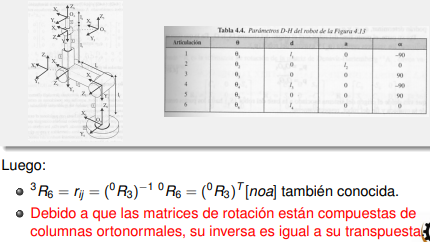
\includegraphics[scale=1]{2.PNG} \\
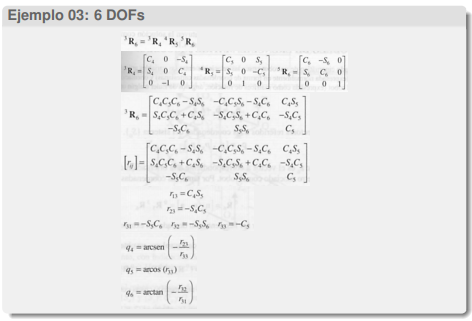
\includegraphics[scale=1]{3.PNG} 
\begin{flushleft}
Resolución mediante el desacoplo cinemático:\\
• Habitualmente los tres último ejes del robot se cortan en un
punto.\\
• La finalidad de estos es lograr la orientación de la herramienta,
aunque como consecuencia de su movimiento tengan un efecto
ligero sobre la posición.\\
• Con la primera condición se puede simplificar enormemente el
problema cinemático para 6 gdl, dado que la obtención de este.\\
punto de intersección intersección es una operación operación sencilla.\\
• Este punto dependerá sólo de los 3 primeros gdl, por lo que su
obtención es asequible.
\begin{flushleft}
Aspectos computacionales: \\
•Para seguimiento de trayectorias es necesario resolver el problema
Aspectos computacionales.\\
•Para seguimiento de trayectorias es necesario resolver el problema.
cinemático a gran velocidad (30 veces/seg o más).\\
•Son pref ibl er es las sol i uc ones cerradas explí i c tas ( is exi ) sten a las
iterativas.\\
•Para acelerar cálculos generalmente se emplean tablas previamente
calculadas (look‐up tables).\\
•El coste de calcular n soluciones, no es necesariamente n veces el de
calcular una única solución.\\
•Computacionalmente es más robusta la arcotangente por lo que es
preferible buscar siempre este tipo de relación.
\begin{flushleft}
Consideraciones
\begin{flushleft}
Deben atenderse las múltiples soluciones:\\
-Elección que minimice los movimientos desde la posición
actual.\\
-Concepto de solución más cercana.\\
-Mover los eslabones de menor peso.\\
-Considerar obstáculos obstáculos (evitar (evitar colisiones).
\begin{flushleft}
Teóricamente Teóricamente es resoluble resoluble todo sistema sistema R y P con 6 grados de
libertad.\\
-Métodos numéricos iterativos: lentitud.\\
-Se prefieren expresiones analíticas (li so uc ones cerrad ) es :\\
-Métodos algebraicos.\\
-Métodos geométricos .
\end{flushleft}
\end{flushleft}
\end{flushleft}
\end{flushleft}
\end{flushleft}
\end{center}
\end{flushleft}
\end{flushleft}
\end{flushleft}

\end{flushleft}
\end{flushleft}
\end{flushleft}
\end{flushleft}
\end{flushleft}
\end{center}
\end{document}